\documentclass{standalone}

% Preamble
\begin{document}

  \subsection{Calcul numérique des racines}

\begin{figure}[h]
    \caption{Processus de réduction exécuté en arithmétique exacte}
  \label{fig:roots}
  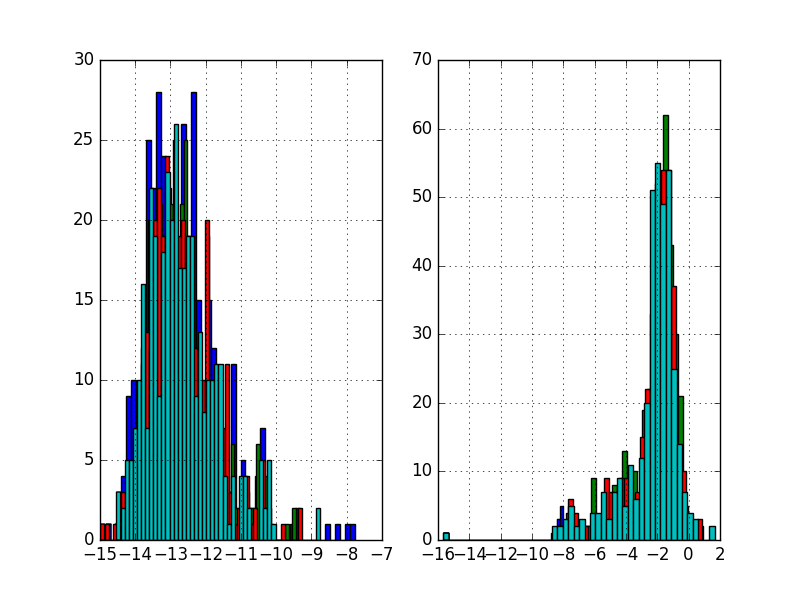
\includegraphics[width=15cm, height=6cm]{../png/roots.png}
\end{figure}
  Nous reprenons l'exemple ci-dessus. La matrice de Bezout $B(1)$, à coefficients entiers, est de taille \input{../txt/Dx.txt}. Après réductions on trouve que la dimension du quotient $A$ est \input{../txt/dim.txt}. En calculant numériquement les valeurs propres des matrices compagnon $X_j = B(x_j)B(1)^{-1}$ on obtient les racines du système polynômial $f$. On vérifie la qualité de chacune des racines obtenues en lui appliquant les polynômes $f_i, i=1,\cdots,n$. Les résultats sont représentés sous forme d'histogramme (Figure \ref{fig:roots}) o\`u le logarithme décimal de l'erreur est porté en abscisse. Sur le plot de gauche le processus de réduction est effectué en arithmétique exacte, sur le plot de droite il est effectué en arithmétique flottante. On constate (Table \ref{tab:timings}) que le temps de calcul en arithmétique flottante est plus court mais au prix d'une dégradation sensible de la qualité des résultats. On peut noter aussi que le calcul de la dimension du quotient, effectué par la méthode des bases de Grobner (fonction vector\_space\_dimension() de Sage), demande un temps beaucoup
plus long que lorsqu'on utilise les matrices de Bezout. Il semble de plus que ce temps de calcul (bases de Grobner) augmente considérablement avec la taille des coefficients entiers du système polynomial, ce qui explique notre choix de restreindre ces coefficients entre $t=-3$ et $t=3$ dans notre expérience.

\begin{table}[h]
    \caption{timings}
\label{tab:timings}
\begin{tabular}{llllr}
  Arithmétique & Méthode & Processus & Software & Timing \\ \hline
  \multirow{4}{*}{flottante} & \multirow{4}{*}{Bezout} & Construction matrices de Bezout & NumPy & $\input{../txt/construction_B_time.txt}$ ms \\ %\hline
  & & Noyau de $B(1)$ & Octave & $\input{../txt/octave_triang_time.txt}$ ms \\
  & & Réduction matrices & Octave & $\input{../txt/octave_reduct_time.txt}$ ms \\ %\hline
  & & Valeurs propres & SciPy & $\input{../txt/eigenstructure_time.txt}$ ms \\ \hline \hline
  \multirow{2}{*}{exacte} & Bezout & Réduction matrices & Sage & $\input{../txt/sage_reduct_time.txt}$ ms \\ %\hline
  & Grobner & Vérification dimension Algèbre & Sage & $\input{../txt/sage_dimension_time.txt}$ ms
\end{tabular}
\end{table}



\end{document}
